\chapter{Experimentos e resultados}
Em linhas gerais, a maior parte do desenvolvimento das frentes de mecânica do projeto se deram de forma tranquila e progressiva, bem como o desenvolvimento do software. A impressão 3D aconteceu de forma planejada e cadenciada, com grande enfoque no desenho e modelagem antes da prototipagem e testes de resistência. 

O desenvolvimento do software também correu bem, na medida do possível, visto que os integrantes do grupo já haviam tido contato com as tecnologias utilizadas na disciplina de Oficina de Integração 1, portanto não ocorreram grandes surpresas no desenvolvimento desta parte do projeto.

Os maiores problemas e consequentes gargalos ocorreram na parte de hardware, com componentes estragando ou não funcionando conforme o esperado sendo os principais destes problemas:
    
\begin{itemize}
  \item GPS com problema: impactou nos testes de hardware fez com que todos demorassem consideravelmente mais, pois era necessário iniciar o cold start do GPS devido a um problema interno em sua bateria.
  \item Segundo GPS com problema: observando os problemas do primeiro GPS, foi comprado um segundo GPS para substituir o antigo, porém este também veio com defeito e não funcionou conforme o esperado, forçando com que fosse utilizado o primeiro novamente.
  \item Bateria com corrente baixa: impactou nos testes do GSM, não conseguimos fazê-lo funcionar pois a corrente fornecida pela bateria era abaixo da mínima requerida pelo GSM. A bateria gerava 800mA e seria necessário no mínimo 1.5A.
  \item Problemas com o powerbank: planejou-se utilizar o powerbank para substituir a bateria pois ele tem uma saida de 5V com 2A, o que em teoria seria o suficiente para todo o projeto. Porém, realizou-se testes e o powerbank não foi suficiente para alimentar o ESP e o GSM, pois continuava não fornecendo energia suficiente.
  \item Queima do OLED: durante a fase final do projeto o OLED queimou e parou de funcionar, assim sendo necessário comprar um novo para a substituição à tempo da entrega.
  \item Possível problema com o Step Down LM2596: durante a fase final do projeto, foi comprada uma fonte de 12V e 10A para alimentar o GSM. O plano era usar o step down para abaixar essa tensao para 4.4V, porém mesmo com essa configuração não foi possivel testar o funcionamento. Outro teste foi realizado utilizando uma fonte regulável da UTFPR e com isso foi possível testar o GSM. Portanto, suspeita-se que o step down estaria prejudicando o funcionamento do GSM.
\end{itemize}

Considerando todas as falhas que ocorreram no projeto, em especial aquelas que envolveram o GSM, optou-se por substituí-lo por Hotspot 4G de um celular Android, visto que a lógica do funcionamento permaneceria coerente. Infelizmente o ESP32 trabalha com redes de 2.4GHz somente, e com celulares Apple isto não seria possível.

Ademais, a integração deu-se baseada sempre em planos paralelos e decisões visando contornar os problemas encontrados na parte de hardware, visando sempre sacrificar o mínimo da integridade e qualidade do projeto possível, mantendo suas funcionalidades.
% testes, integração, etc.

\section{Software}
O software para a API foi desenvolvido com base no proposto para o projeto, através do NodeJS e MongoDB, onde as localizações estão sendo salvas e posteriormente acessadas, como demonstrado na Figura \ref{fig:mongodb-locations}.

\begin{figure}[!h]
\centering
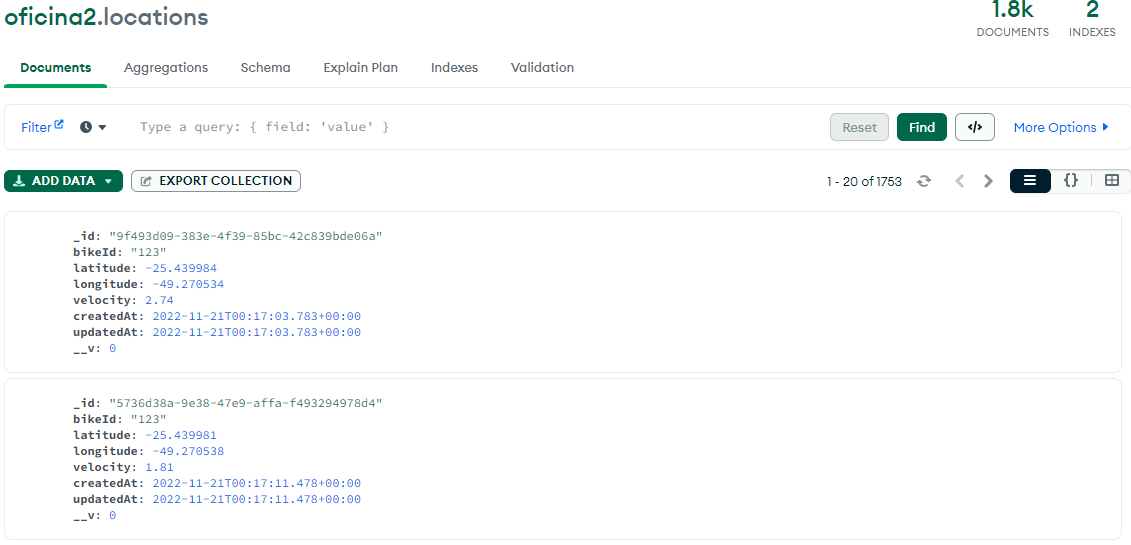
\includegraphics[width=15cm]{capitulos/Figuras/mongo-locations.png}
\caption{Localizações salvas no Banco de Dados.}
\label{fig:mongodb-locations}
\end{figure}

O software para o aplicativo também foi desenvolvido com as tecnologias propostas, através de Flutter com foco no Android. O aplicativo é constituído de um mapa com uma gaveta de navegação para poder ver as bicicletas do usuário e/ou amigo, demonstrado na Figura \ref{fig:app-map}. O dono da bicicleta tem o permissionamento para estacionar a bicicleta, permissão qual o amigo não tem, demonstrados nas Figuras \ref{fig:app-owner} e \ref{fig:app-buddy} respectivamente.

\begin{figure}[!h]
\centering
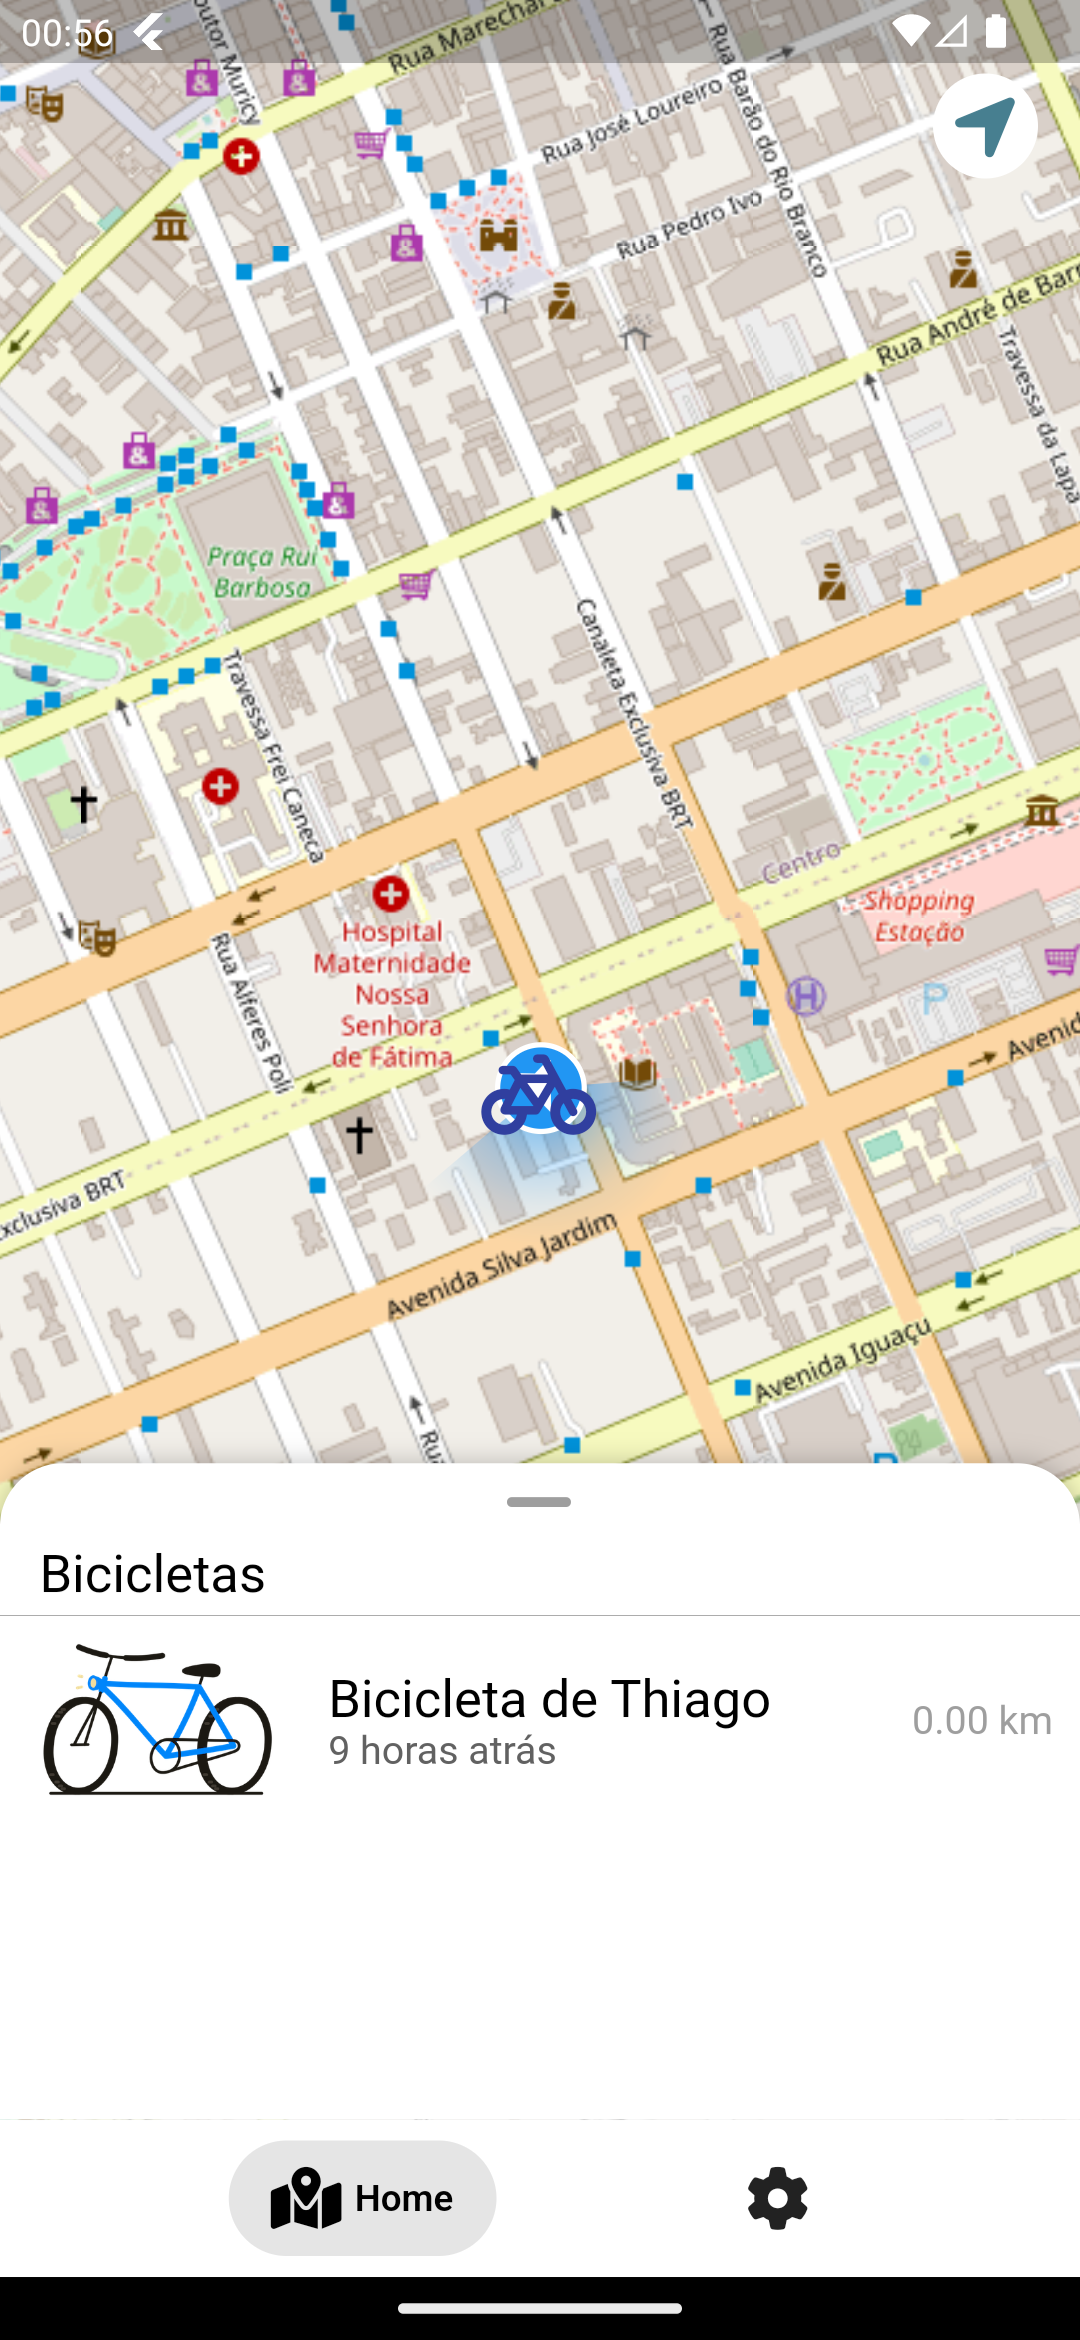
\includegraphics[width=8cm]{capitulos/Figuras/app-map.png}
\caption{Visão das bicicletas disponíveis no mapa.}
\label{fig:app-map}
\end{figure}

\newpage

\begin{figure}[!h]
\centering
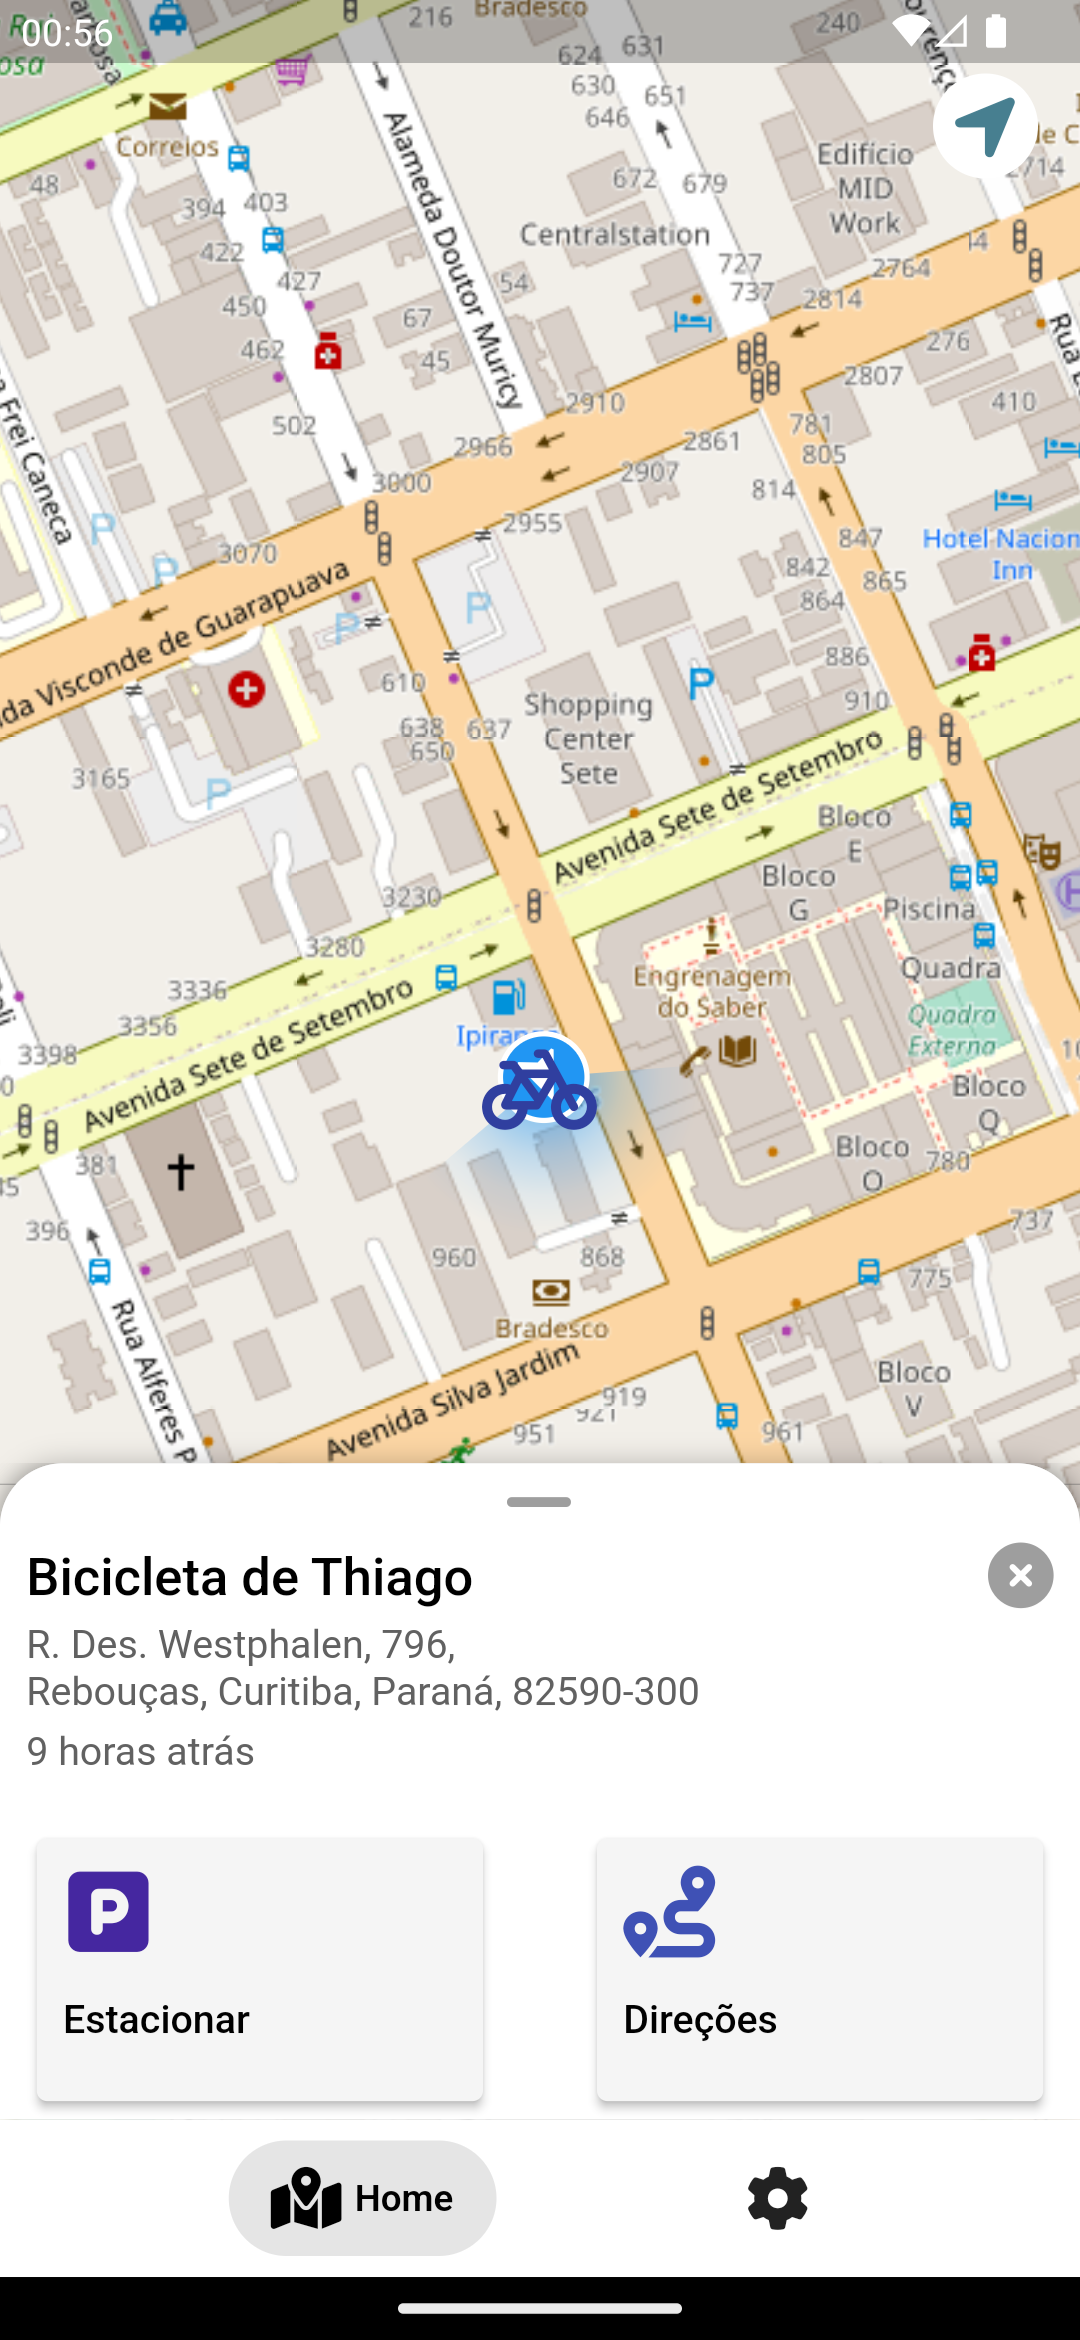
\includegraphics[width=8cm]{capitulos/Figuras/app-owner.png}
\caption{Visão do dono da bicicleta.}
\label{fig:app-owner}
\end{figure}

\newpage

\begin{figure}[!h]
\centering
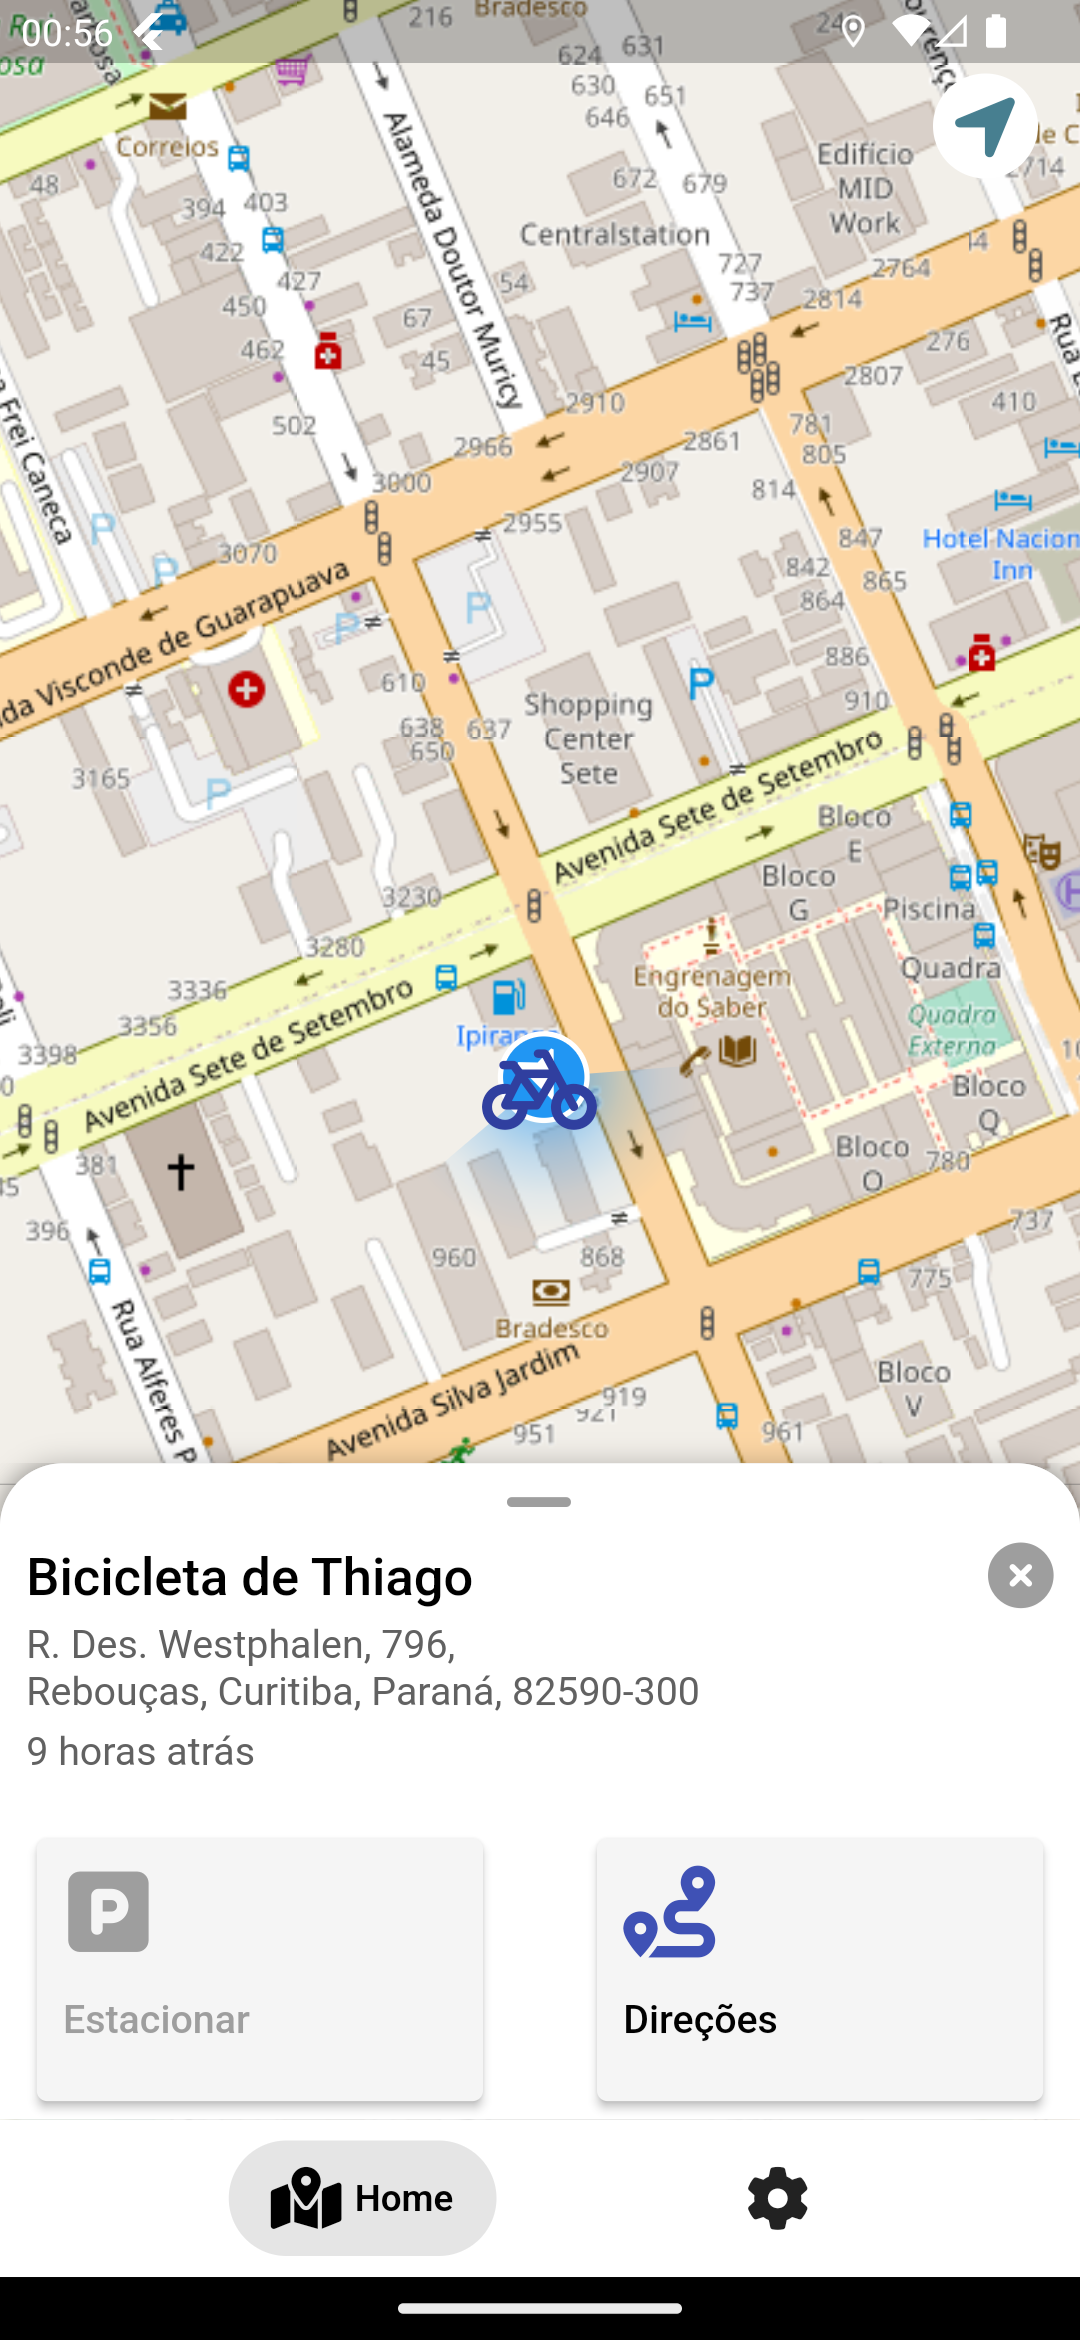
\includegraphics[width=8cm]{capitulos/Figuras/app-buddy.png}
\caption{Visão do amigo.}
\label{fig:app-buddy}
\end{figure}

\section{Hardware}

    O hardware foi montado em uma placa perfurada conforme o circuito demonstrado na Figura \ref{fig:diagrama_hardware} foi soldado diversos pinos na placa com o intuito de deixa-la modular, ou seja caso ocorra a queima de algum componente ele pode ser facilmente retirado da placa para a substituição como demonstrado na Figura \ref{fig:hardware_placa} e \ref{fig:hardware_pinos}.
    
\begin{figure}[!h]
\centering
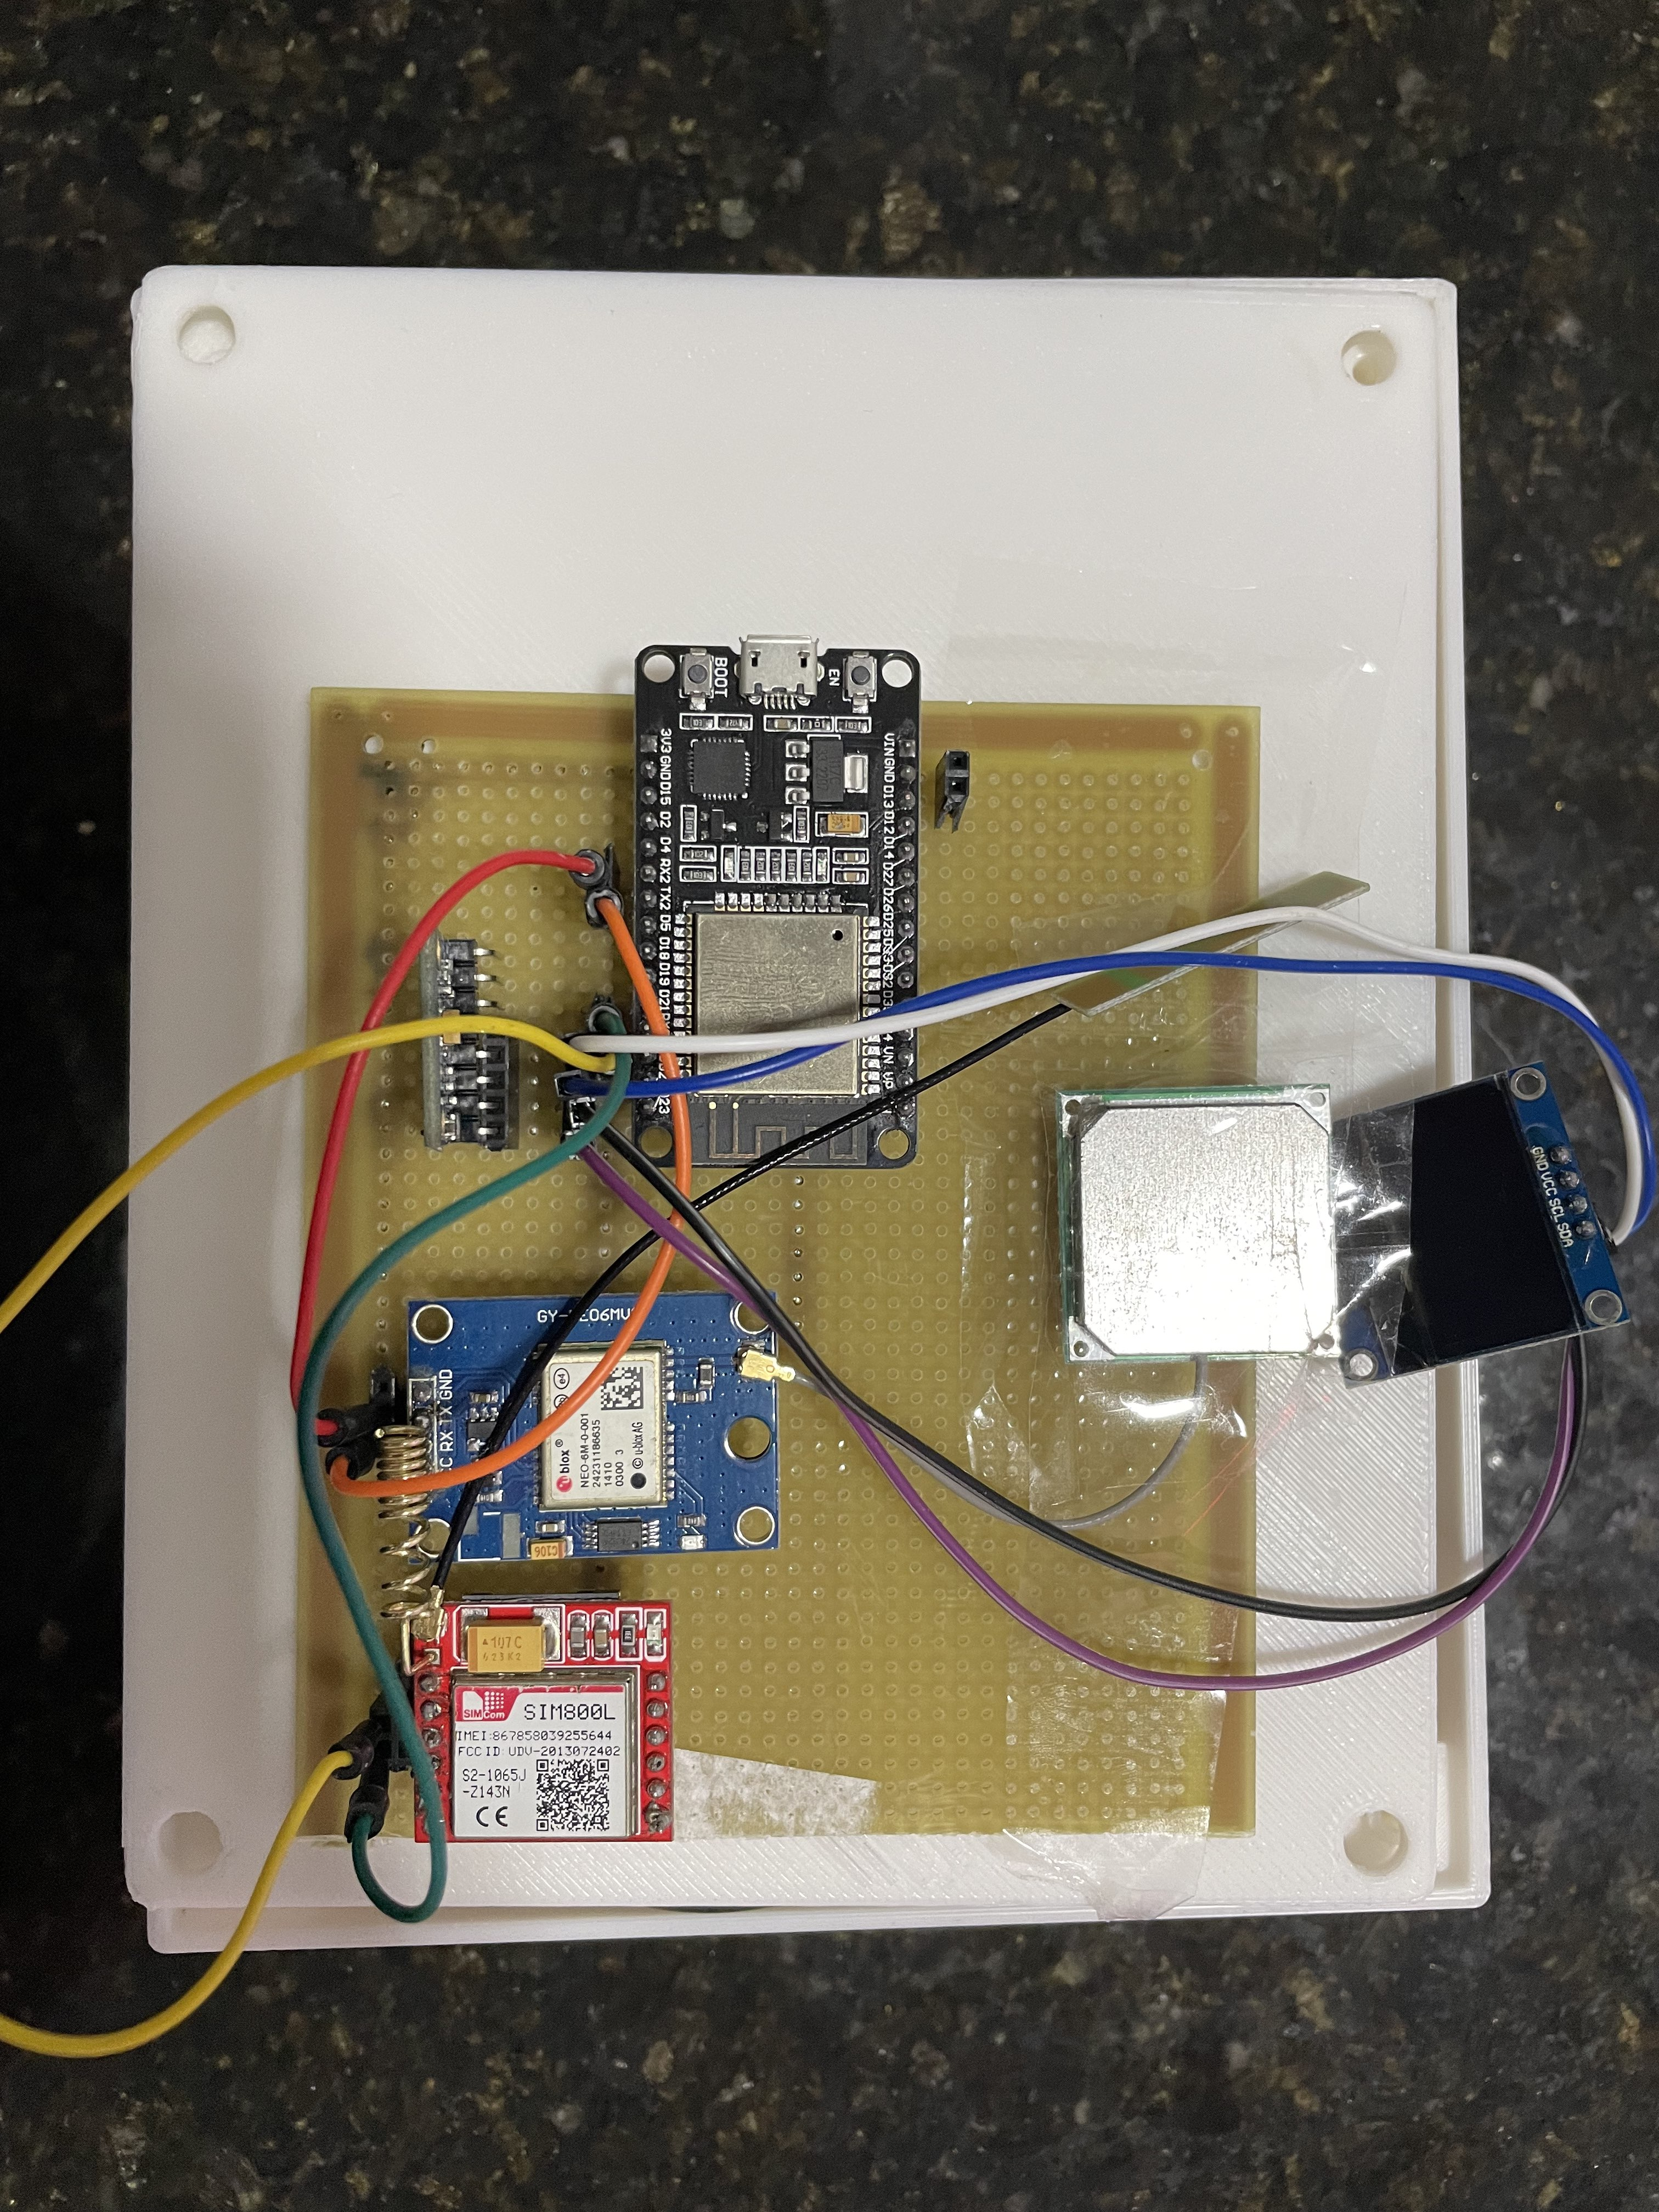
\includegraphics[width=10cm, height = 10cm]{capitulos/Figuras/Imagem_Hardware_2.jpg}
\caption{Placa perfurada.}
\label{fig:hardware_placa}
\end{figure}

\begin{figure}[!h]
\centering
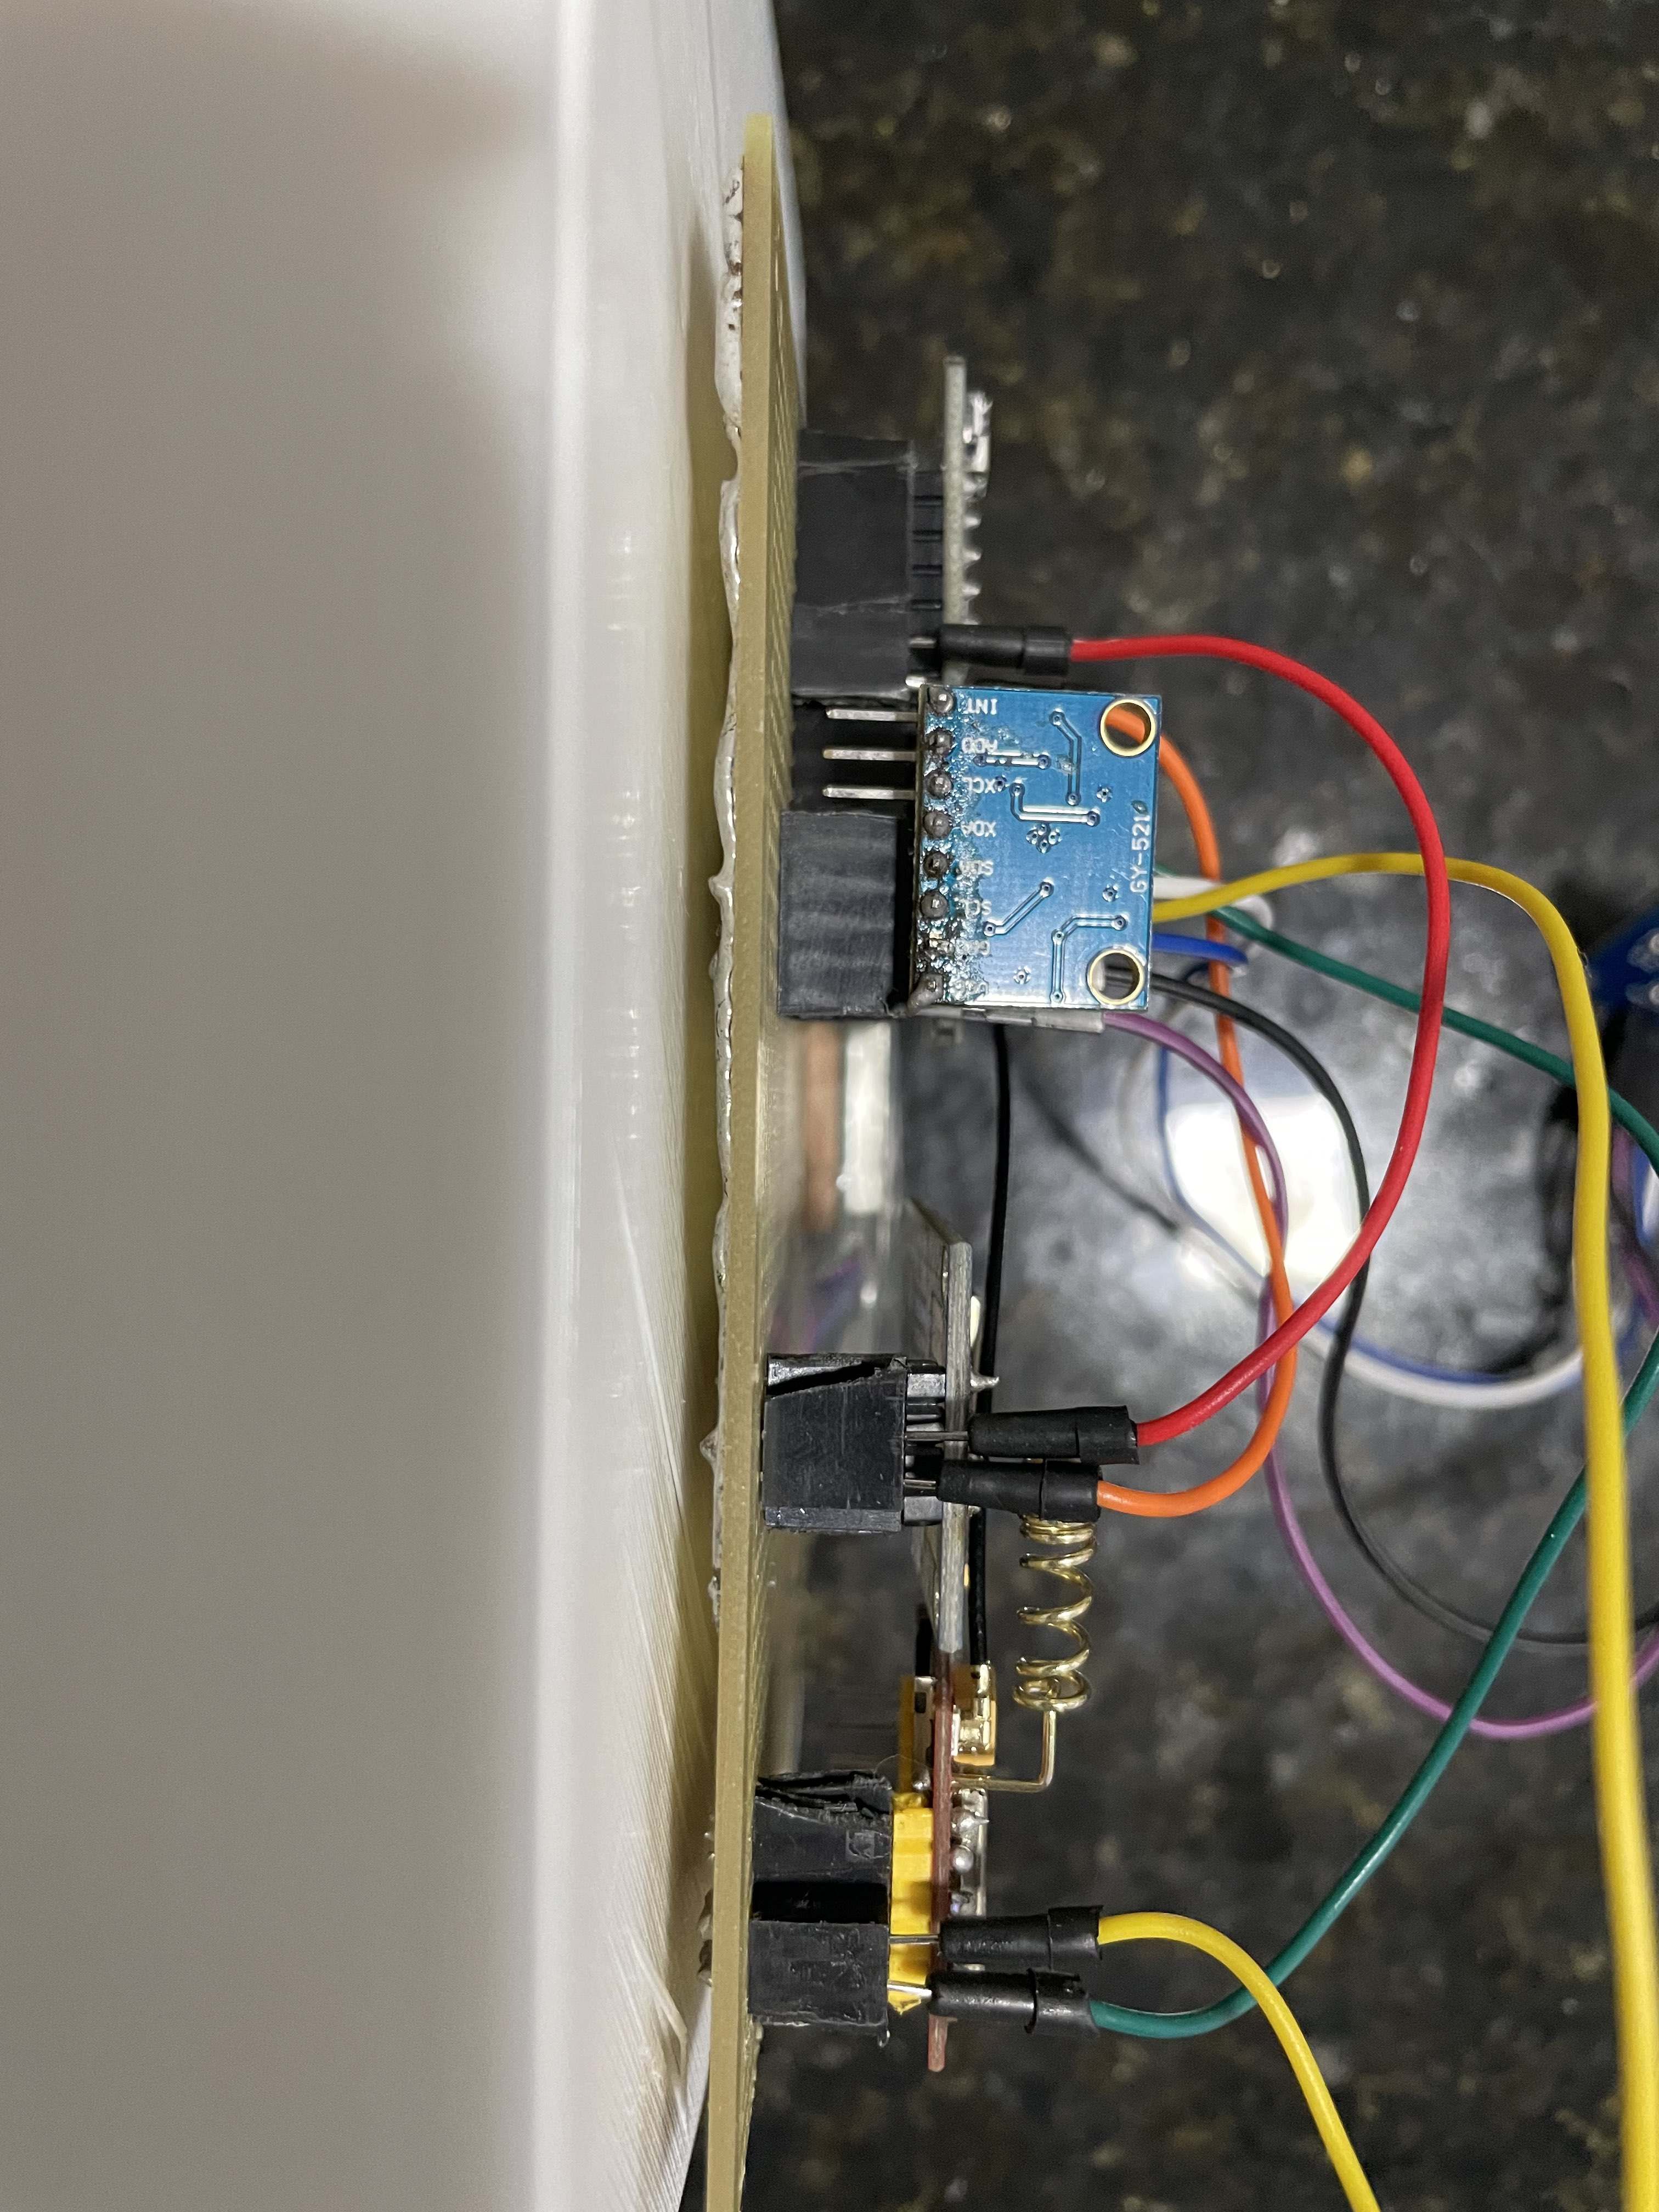
\includegraphics[width=10cm, height = 10cm]{capitulos/Figuras/Imagem_Hardware_1.jpg}
\caption{Placa perfurada pinos.}
\label{fig:hardware_pinos}
\end{figure}

